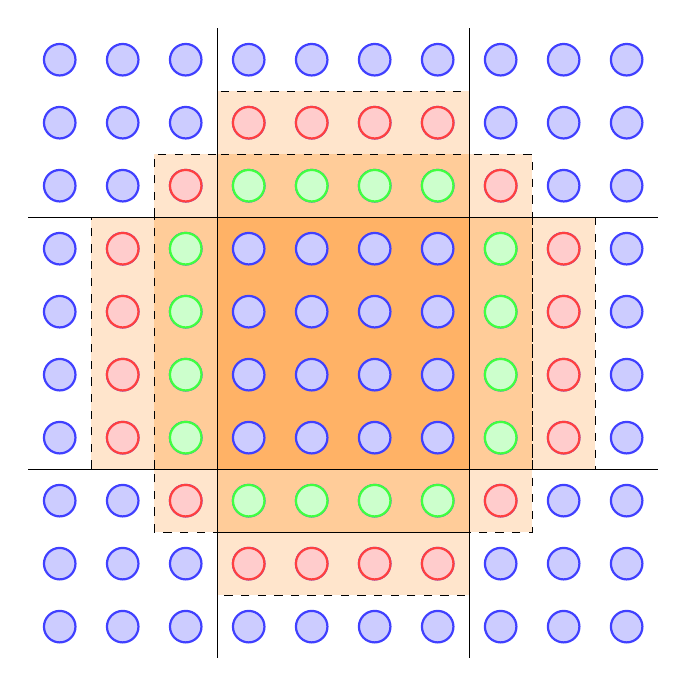
\begin{tikzpicture}[scale=0.8]
\tikzstyle{place1}=[circle,thick,draw=blue!75,fill=blue!20,minimum size=4mm]
\tikzstyle{place2}=[circle,thick,draw=green!75,fill=green!20,minimum size=4mm]
\tikzstyle{place3}=[circle,thick,draw=red!75,fill=red!20,minimum size=4mm]

\draw[dashed,fill=orange!20] (2.5,7.5) rectangle (6.5,8.5);
\draw[dashed,fill=orange!20] (2.5,0.5) rectangle (6.5,1.5);

\draw[dashed,fill=orange!20] (1.5,6.5) rectangle (0.5,2.5);
\draw[dashed,fill=orange!20] (8.5,6.5) rectangle (7.5,2.5);

\draw[dashed,fill=orange!20] (1.5,1.5) rectangle (7.5,7.5);


\draw[dashed,fill=orange!40] (2.5,6.5) rectangle (6.5,7.5);
\draw[dashed,fill=orange!40] (2.5,1.5) rectangle (6.5,2.5);

\draw[dashed,fill=orange!40] (2.5,6.5) rectangle (1.5,2.5);
\draw[dashed,fill=orange!40] (7.5,6.5) rectangle (6.5,2.5);


\draw[fill=orange!60] (2.5,2.5) rectangle (6.5,6.5);


\draw (2.5,2.5) -- (-0.5,2.5);
\draw (6.5,2.5) -- (9.5,2.5);

\draw (2.5,6.5) -- (-0.5,6.5);
\draw (6.5,6.5) -- (9.5,6.5);


\draw (2.5,2.5) -- (2.5,-0.5);
\draw (2.5,6.5) -- (2.5,9.5);

\draw (6.5,2.5) -- (6.5,-0.5);
\draw (6.5,6.5) -- (6.5,9.5);


\foreach \x in {0,...,9}
{
  \foreach \y in {0,...,9}
  {
    \node[place1] () at (\x,\y) {};
  }
}

\foreach \x in {3,...,6}
{
  \node[place2] () at (\x,2) {};
  \node[place2] () at (\x,7) {};
}
\foreach \y in {3,...,6}
{
  \node[place2] () at (2,\y) {};
  \node[place2] () at (7,\y) {};
}


\foreach \x in {3,...,6}
{
  \node[place3] () at (\x,1) {};
  \node[place3] () at (\x,8) {};
}
\foreach \y in {3,...,6}
{
  \node[place3] () at (1,\y) {};
  \node[place3] () at (8,\y) {};
}


\node[place3] () at (2,2) {};
\node[place3] () at (7,2) {};
\node[place3] () at (2,7) {};
\node[place3] () at (7,7) {};


\end{tikzpicture}
